\documentclass[12pt]{article}
\usepackage[paper=letterpaper,margin=2cm]{geometry}
\usepackage{amsmath,amssymb,amsfonts}
\usepackage{enumitem}
\usepackage{titling}
\usepackage{multirow}
\usepackage{xcolor}
\usepackage{float}
\usepackage{graphicx}
\usepackage{xcolor}
\usepackage[colorlinks=true, linkcolor=red]{hyperref}
\usepackage{subcaption} % For subfigures
\usepackage{adjustbox}  % For centering the bottom image
\usepackage{listings}
\usepackage{xcolor} % For setting colors
\usepackage{booktabs} % For better tables
\usepackage{threeparttable} % For table notes

\usepackage{listings}
\usepackage{xcolor}

\definecolor{codegreen}{rgb}{0.0, 0.514, 0.325}      
\definecolor{codegray}{rgb}{0.75, 0.75, 0.75}    
\definecolor{codeblue}{rgb}{0.122, 0.467, 0.706}  
\definecolor{extraLightGray}{rgb}{0.98, 0.98, 0.98}
\definecolor{codepink}{rgb}{0.894, 0.0, 0.443}

\lstdefinestyle{mystyle}{
    backgroundcolor=\color{extraLightGray},
    commentstyle=\color{codegreen},
    keywordstyle=\color{codeblue},
    numberstyle=\tiny\color{codegray},
    stringstyle=\color{codepink},
    basicstyle=\ttfamily\footnotesize,
    breakatwhitespace=false,
    breaklines=true,
    captionpos=b,
    keepspaces=true,
    numbers=left,
    numbersep=5pt,
    showspaces=false,
    showstringspaces=false,
    showtabs=false,
    tabsize=2
}
\lstset{style=mystyle}

\setlength{\droptitle}{-6em}

\begin{document}

\begin{center}
Aprendizagem 2023\\
Homework I --- Group 003\\
(ist1107028, ist1107137)\vskip 1cm
\end{center}

\large{\textbf{Part I}: Pen and paper}\normalsize

\vspace{10pt}
\textbf{For questions in this group, show your numerical results with 5 decimals or scientific notation.
Hint: we highly recommend the use of \texttt{numpy} (e.g., \texttt{linalg.pinv} for inverse) or other programmatic
facilities to support the calculus involved in both questions (1) and (2).}

\textbf{Below is a training dataset $\mathbf{D}$ composed by two input variables and two output variables, one of 
which is numerical ($\mathbf{y_{num}}$) and the other categorical ($\mathbf{y_{class}}$) . Consider a polynomial basis function
$\mathbf{\phi(y_1,y_2) = y_1 \times y_2}$ that transforms the original space into a new one-dimensional space.}

\begin{table}[H]
    \begin{center}
        \begin{tabular}{c|cc|cc}
            D & $y_1$ & $y_2$ & $y_{\text{num}}$ & $y_{\text{class}}$ \\
            \hline
            $x_1$ & 1 & 1 & 1.25 & B \\
            $x_2$ & 1 & 3 & 7.0 & A \\
            $x_3$ & 3 & 2 & 2.7 & C \\
            $x_4$ & 3 & 3 & 3.2 & A \\
            $x_5$ & 2 & 4 & 5.5 & B \\
        \end{tabular}
    \end{center}
\end{table}

\begin{enumerate}
    \item \textbf{Learn a regression model on the transformed feature space using the OLS closed form
    solution to predict the continuous output variable $\mathbf{y_{\text{num}}}$.}
    
    \vspace{10pt}
    The first step will be to calculate the transformed feature space for each observation using the polynomial basis function:
    
    \begin{equation}\label{eq:phi}
        \phi(y_1, y_2) = y_1 \times y_2
    \end{equation}

    By applying \eqref{eq:phi} to each observation, we get:

    \begin{equation*}
        \begin{aligned}
            \phi(x_1) &= 1 \times 1 = 1 \qquad \phi(x_2) = 1 \times 3 = 3 \qquad \phi(x_3) = 3 \times 2 = 6\\
            \phi(x_4) &= 3 \times 3 = 9 \qquad \phi(x_5) = 2 \times 4 = 8 \\
        \end{aligned}
    \end{equation*}

    \vspace{10pt}
    We end up with the following transformed feature space: $\phi(y_1, y_2) = [1, 3, 6, 9, 8]$
    
    \vspace{10pt}
    The regression model in the transformed feature space is given by:
    
    \begin{equation*}
        z = w_0 + w_1 \cdot \phi(y_1, y_2)
    \end{equation*}

    \vspace{10pt}
    The next step is to learn a regression model using the OLS closed form solution which, for this exercise, is given by:
    \begin{equation*}
        W = (\Phi^T \Phi)^{-1} \Phi^T y_\text{num}
    \end{equation*}

    where $\Phi$ is the parameterization matrix and $y_\text{num}$ is the output variable. 

    \begin{equation*}
        \Phi = \begin{bmatrix}
            1 & 1 \\
            1 & 3 \\
            1 & 6 \\
            1 & 9 \\
            1 & 8
        \end{bmatrix} \qquad
        y_\text{num} = \begin{bmatrix}
            1.25 \\
            7.0 \\
            2.7 \\
            3.2 \\
            5.5
        \end{bmatrix}
    \end{equation*}

    As suggested in the hint, we will use \texttt{numpy} to calculate the weights $W$:

    \vspace{10pt}
    \lstinputlisting[language=Python]{./Part I/1.py}

    \vspace{10pt}
    The output of the code above is $[3.31593\text{ }0.11372]$.\\ 
    Therefore, the weights are $w_0 = 3.31593$ and $w_1 = 0.11372$.

    \vspace{10pt}
    The regression model is then given by:
    \begin{equation*}
        y_\text{num} = 3.31593 + 0.11372 \cdot \phi(y_1, y_2)
    \end{equation*}

    \item \textbf{Repeat the previous exercise, but this time learn a Ridge regression with penalty
    factor $\mathbf{\lambda = 1}$. Compare the learnt coefficients with the ones from the previous exercise and
    discuss how regularization affects them.}

    \vspace{10pt}
    The Ridge regression model is given by:
    \begin{equation*}
        W = (\Phi^T \Phi + \lambda I)^{-1} \Phi^T y_\text{num}
    \end{equation*}
    
    where $\Phi$ is the parameterization matrix, $y_\text{num}$ is the output variable (which remain the same as in the previous exercise), and $\lambda$ is the penalty factor.

    \vspace{10pt}
    \lstinputlisting[language=Python]{./Part I/2.py}

    \vspace{10pt}
    The output of the code above is $[1.81809\text{ }0.32376]$.\\
    Therefore, the weights are $w_0 = 1.81809$ and $w_1 = 0.32376$.

    \vspace{10pt}
    The Ridge regression model is then given by:
    \begin{equation*}
        y_\text{num} = 1.81809 + 0.32376 \cdot \phi(y_1, y_2)
    \end{equation*}

    In order to compare the weights obtained in the OLS and Ridge regression models, we must first normalize the data:

    \vspace{10pt}
    normalization for the OLS model:
    \begin{equation*}
        \begin{aligned}
            {w_0}_\text{normalized} &= \frac{3.31593}{3.31593 + 1.81809} = 0.64587 \\
            {w_1}_\text{normalized} &= \frac{0.11372}{0.11372 + 0.32376} = 0.25994
        \end{aligned}
    \end{equation*}

    \vspace{10pt}
    Normalization for the Ridge Regression model:
    \begin{equation*}
        \begin{aligned}
            {w_0}_\text{normalized} &= \frac{1.81809}{3.31593 + 1.81809} = 0.35413 \\
            {w_1}_\text{normalized} &= \frac{0.32376}{0.11372 + 0.32376} = 0.74006
        \end{aligned}
    \end{equation*}

    \vspace{10pt}
    Comparing the normalized weights obtained in the OLS and Ridge regression models, we can see that in the Ridge regression model $w_0$ is smaller and $w_1$ is larger than the corresponding OLS model weights.

    The regularization term in the Ridge regression model penalizes large weights, but it allows for the weights to increase or decrease relative to one another based on the data. In this case, the regularization reduces the bias term $w_0$, as the model learns to rely more on the feature $w_1$
    to explain the variance in the target variable. This reduces the need for a large bias term, helping to prevent overfitting and stabilizing the model's predictions.

    These results suggest that the feature has a strong positive correlation with the target variable. As a result, $w_1$ increases to better capture this relationship, allowing $w_0$
    to decrease.

    \vspace{10pt}
    \item \textbf{Given three new test observations and their corresponding output\\}
    $\mathbf{x_6 = (2,2,0.7), x_7 = (1,2,1.1),}$ \textbf{ and } $\mathbf{x_8 = (5,1,2.2),}$
    \textbf{compare the train and test RMSE of the two models obtained in (1) and (2). Explain if the results go according to what is expected.}    

    \vspace{10pt}
    The Root Mean Squared Error (RMSE) is given by:
    \begin{equation*}
        \text{RMSE} = \sqrt{\frac{1}{N} \sum_{i=1}^{N} (z_{i} - \tilde{z}_{i})^2}
    \end{equation*}

    where $\tilde{z}_{i}$ is the predicted value, $z_{i}$ is the true value and $N$ is the number of observations.

    \vspace{10pt}
    \underline{OLS model:}

    \vspace{10pt}
    Using the values of the weights obtained in the first exercise, we can calculate the predicted values for all observations:
    \begin{equation*}
        \footnotesize
        \underbrace{
        \Phi = \begin{bmatrix}
            1 & 1 \\
            1 & 3 \\
            1 & 6 \\
            1 & 9 \\
            1 & 8 
        \end{bmatrix} \land w = \begin{bmatrix}
            3.31593 \\
            0.11372
        \end{bmatrix} \Rightarrow \tilde{z} = \begin{bmatrix}
            3.42965 \\
            3.65709 \\
            3.99825 \\
            4.33941 \\
            4.22569
        \end{bmatrix} }_{\text{\colorbox{codeblue}{\textcolor{white}{train observations}}}}
        \quad \underbrace{
            \Phi = \begin{bmatrix}
            1 & 4 \\
            1 & 2 \\
            1 & 5 
        \end{bmatrix} \land w = \begin{bmatrix}
            3.31593 \\
            0.11372
        \end{bmatrix} \Rightarrow \tilde{z} = \begin{bmatrix}
            3.77081 \\
            3.54337 \\
            3.88453
        \end{bmatrix}
        }_{\text{\colorbox{codepink}{\textcolor{white}{test observations}}}}
    \end{equation*}

    Finally, we take $z = [\textcolor{codeblue}{1.25}, \textcolor{codeblue}{7.0}, \textcolor{codeblue}{2.7}, \textcolor{codeblue}{3.2}, \textcolor{codeblue}{5.5}, \textcolor{codepink}{0.7}, \textcolor{codepink}{1.1}, \textcolor{codepink}{2.2}]$ along with the predicted values to calculate the two RMSE for the OLS model.

    \begin{equation*}
        \text{RMSE}_{\text{train}(x_1\--x_5)} = \sqrt{\frac{1}{5} \sum_{i=1}^{5} (z_{i} - \tilde{z}_{i})^2} = \sqrt{\frac{1}{5} \times 25.0637837} = 2.2389
    \end{equation*}

    \begin{equation*}
        \text{RMSE}_{\text{test}(x_6\--x_8)} = \sqrt{\frac{1}{3} \sum_{i=1}^{3} (z_{i} - \tilde{z}_{i})^2} = \sqrt{\frac{1}{3} \times 18.23757233} = 2.4656
    \end{equation*}
    
    \vspace{10pt}
    \underline{Ridge Regression model:}

    \vspace{10pt}
    Repeating the exact same process for the Ridge model, we get the following predicted values:
    \begin{equation*}
        \footnotesize
        \underbrace{
        \Phi = \begin{bmatrix}
            1 & 1 \\
            1 & 3 \\
            1 & 6 \\
            1 & 9 \\
            1 & 8 
        \end{bmatrix} \land w = \begin{bmatrix}
            1.81809 \\
            0.32376
        \end{bmatrix} \Rightarrow \tilde{z} = \begin{bmatrix}
            2.14185 \\
            2.78937 \\
            3.76065 \\
            4.73193 \\
            4.40817
        \end{bmatrix}
        }_{\text{\colorbox{codeblue}{\textcolor{white}{train observations}}}}
        \quad \underbrace{
            \Phi = \begin{bmatrix}
            1 & 4 \\
            1 & 2 \\
            1 & 5 
        \end{bmatrix} \land w = \begin{bmatrix}
            1.81809 \\
            0.32376
        \end{bmatrix} \Rightarrow \tilde{z} = \begin{bmatrix}
            3.11313 \\
            2.46561 \\
            3.43689
        \end{bmatrix}
        }_{\text{\colorbox{codepink}{\textcolor{white}{test observations}}}}
    \end{equation*}
    
    We take $z = [\textcolor{codeblue}{1.25}, \textcolor{codeblue}{7.0}, \textcolor{codeblue}{2.7}, \textcolor{codeblue}{3.2}, \textcolor{codeblue}{5.5}, \textcolor{codepink}{0.7}, \textcolor{codepink}{1.1}, \textcolor{codepink}{2.2}]$ along with the predicted values to calculate the RMSE for the Ridge model.

    \begin{equation*}
        \text{RMSE}_{\text{train}(x_1\--x_5)} = \sqrt{\frac{1}{5} \sum_{i=1}^{5} (z_{i} - \tilde{z}_{i})^2} = \sqrt{\frac{1}{5} \times 23.18868212} = 2.1535
    \end{equation*}
 
    \begin{equation*}
        \text{RMSE}_{\text{test}(x_6\--x_8)} = \sqrt{\frac{1}{3} \sum_{i=1}^{3} (z_{i} - \tilde{z}_{i})^2} = \sqrt{\frac{1}{3} \times 9.217983941} = 1.7529
    \end{equation*}

    \vspace{20pt}
    Comparing the RMSE values for the train and test observations, we can see that the Ridge regression model has a lower RMSE for both the train and test data compared to the OLS model. This suggests that the Ridge regression model makes more accurate predictions and fits the data better than the OLS model. The regularization term in the Ridge regression model helps to prevent overfitting and improve the generalization of the model to new data, resulting in lower prediction errors.

    \vspace{10pt}
    \item \textbf{Consider an MLP to predict the output $\mathbf{y_\text{class}}$ characterized by the weights}
    
    \[
W^{[1]} = \begin{bmatrix}
0.1 & 0.1 \\
0.1 & 0.2 \\
0.2 & 0.1
\end{bmatrix}, \quad
b^{[1]} = \begin{bmatrix}
0.1 \\
0 \\
0.1
\end{bmatrix}, \quad
W^{[2]} = \begin{bmatrix}
1 & 2 & 2 \\
1 & 2 & 1 \\
1 & 1 & 1
\end{bmatrix}, \quad
b^{[2]} = \begin{bmatrix}
1 \\
1 \\
1
\end{bmatrix}
\]

\textbf{the output activation function}

\begin{equation*}
    \text{softmax}(z_c^\text{[out]}) = \frac{e^{z_c^\text{[out]}}}{\sum_{l=1}^{|C|} e^{z_c^\text{[out]}}}
\end{equation*}

\textbf{, no activations on the hidden layer(s) and the cross-entropy loss:}

\begin{equation}\label{eq:CE}
    \text{CE} = -\sum_{i=1}^{N}\sum_{l=1}^{|C|} t_{l}^{\text{(i)}} \log(X_{l}^{\text{[out](i)}})
\end{equation}

\textbf{Consider also that the output layer of the MLP gives the predictions for the classes A, B and C in this order. Perform one
stochastic gradient descent update to all the weights and biases with learning rate $\eta = 0.1$
using the training observation $x_1$.}

\begin{figure}[H]
    \centering
    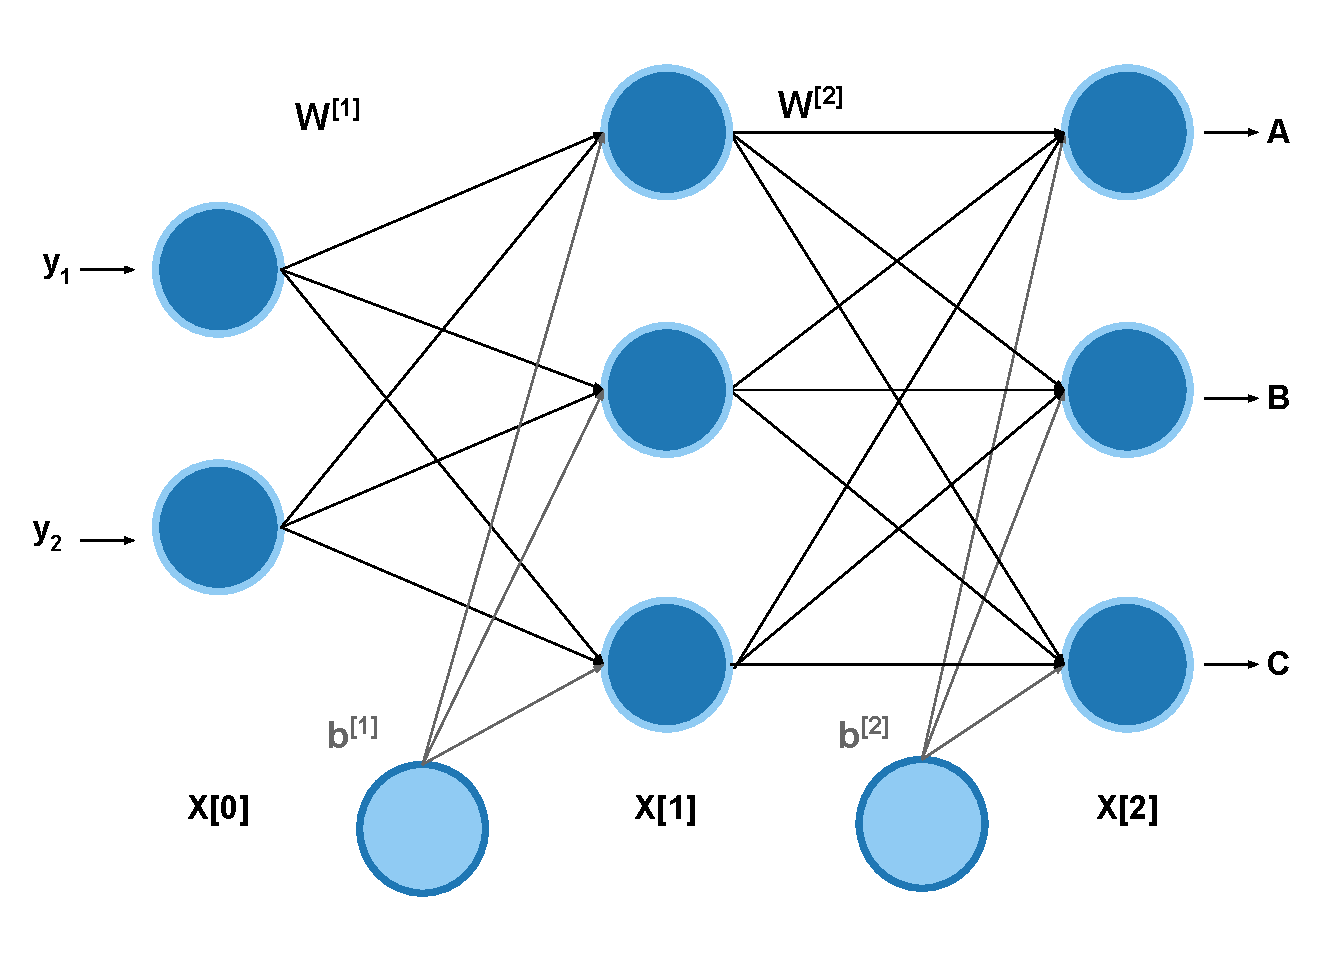
\includegraphics[width=12cm]{./Part I/MLP_corrected.pdf}
    \caption{MLP architecture}
\end{figure}

\vspace{10pt}
We may also draw the corresponding scheme:
\begin{figure}[H]
    \centering
    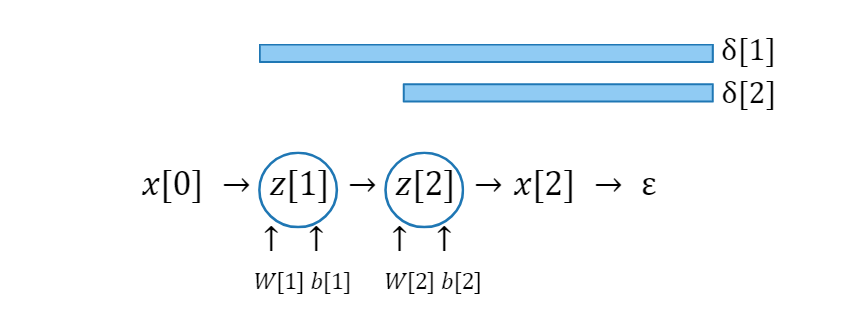
\includegraphics[width=12cm]{./Part I/Scheme.png}
    \caption{MLP Scheme}
\end{figure}

To begin, we initiate the process with the \textbf{forward propagation}. Below are the key equations to calculate the values of each
layer, $x^{[p]}_i$:

\begin{align*}
z^{[p]}_i = W^{[p]} \, x^{[p-1]}_i + b^{[p]} & \qquad\qquad
x^{[p]}_i = f\left(z^{[p]}_i\right)
\end{align*}

$f$ is the activation function for the output layer, provided in the statement.

\begin{equation*}
    f = \text{softmax}(z_c^\text{[out]}) = \frac{e^{z_c^\text{[out]}}}{\sum_{l=1}^{|C|} e^{z_c^\text{[out]}}}
\end{equation*}

\vspace{10pt}
In this notation, the value $p$ is the index of the MLP layer.

We may now calculate the values of each node in the network for the training observation:

\vspace{10pt}
\fbox{$x_1$}
\begin{equation*}
    \begin{aligned}
        z^{[1]} &= W^{[1]} \, x^{[0]} + b^{[1]} = \begin{bmatrix}
            0.1 & 0.1 \\
            0.1 & 0.2 \\
            0.2 & 0.1
        \end{bmatrix} \begin{bmatrix}
            1 \\
            1
        \end{bmatrix} + \begin{bmatrix}
            0.1 \\
            0 \\
            0.1
        \end{bmatrix} = \begin{bmatrix}
            0.3 \\
            0.3 \\
            0.4
        \end{bmatrix} \\
        x^{[1]} &= z^{[1]} = \begin{bmatrix}
            0.3 \\
            0.3 \\
            0.4
        \end{bmatrix}
    \end{aligned}
\end{equation*}

\begin{equation*}
    \begin{aligned}
        z^{[2]} &= W^{[2]} \, z^{[1]} + b^{[2]} = \begin{bmatrix}
            1 & 2 & 2 \\
            1 & 2 & 1 \\
            1 & 1 & 1
        \end{bmatrix} \begin{bmatrix}
            0.3 \\  
            0.3 \\
            0.4 \\
        \end{bmatrix} + \begin{bmatrix}
            1 \\
            1 \\
            1
        \end{bmatrix} = \begin{bmatrix}
            2.7 \\
            2.3 \\
            2.0
        \end{bmatrix} \\
        x^{[2]} &= f\left(z^{[2]}\right) = \begin{bmatrix}
            0.461 \\
            0.309 \\
            0.229
        \end{bmatrix}
    \end{aligned}
\end{equation*}

\vspace{10pt}
Now, we can calculate the \textbf{backward propagation} to update the weights and biases.

\newpage
Let's star by computing the derivatives for the z[i]:
    
    \begin{equation*}
        \begin{aligned}
            &\frac{\partial z^{[i]}(W^{[i]}, b^{[i]}, x^{[i-1]})}{\partial W^{[i]}} = x^{[i-1]}\\
            &\frac{\partial z^{[i]}(W^{[i]}, b^{[i]}, x^{[i-1]})}{\partial b^{[i]}} = 1 \qquad \quad \quad \frac{\partial z^{[i]}(W^{[i]}, b^{[i]}, x^{[i-1]})}{\partial x^{[i-1]}} = W^{[i]}\\
        \end{aligned}
    \end{equation*}

\vspace{10pt}
Now we calculate the deltas (for the output layer and the hidden layer):

\begin{equation*}
    \begin{aligned}
        \delta^{[2]} &= \mathbf{x}^{[2]} - t\\
        \\
        &= \begin{pmatrix} 
            0.461 \\
            0.309 \\
            0.229
            \end{pmatrix} -
            \begin{pmatrix} 
            0\\     
            1\\
            0 
            \end{pmatrix} = \begin{pmatrix}
            0.461 \\
            -0.691 \\
            0.229 
            \end{pmatrix}\\
        \\
        \delta^{[1]} &= \left(\frac{\partial \mathbf{z}^{[2]}}{\partial \mathbf{x}^{[1]}}\right)^T \cdot \delta^{[2]} = \left(\mathbf{W}^{[2]}\right)^T \cdot \delta^{[2]}\\
        \\
        &= \begin{pmatrix}
            1 & 1 & 1\\
            2 & 2 & 1\\
            2 & 1 & 1
        \end{pmatrix} \cdot \begin{pmatrix}
            0.461 \\
            -0.691 \\
            0.229 
        \end{pmatrix} \circ \begin{pmatrix}
            0.3\\
            0.3\\
            0.4
        \end{pmatrix} = \begin{pmatrix}
            -0.001\\
            -0.231\\
            0.460
        \end{pmatrix} 
    \end{aligned}
\end{equation*}

\vspace{10pt}
Finally, we can \textbf{update the weights and biases} with the gradient descent:

\begin{equation*}
    \begin{aligned}
        \frac{\partial E}{\partial \mathbf{W}^{[1]}} &= \delta^{[1]} \cdot \frac{\partial \mathbf{z}^{[1]}}{\partial \mathbf{W}^{[1]}} = \delta^{[1]} \cdot \left(\mathbf{x}^{[0]}\right)^T \\
        &= \begin{pmatrix}
            -0.001\\
            -0.231\\
            0.460
        \end{pmatrix} \cdot \begin{pmatrix}
            1 & 1 
        \end{pmatrix} = \begin{pmatrix}
            -0.001 & -0.001\\
            -0.231 & -0.231\\
            0.460 & 0.460
        \end{pmatrix}\\
        \\
        \mathbf{W}^{[1]} &= \mathbf{W}^{[1]} - \eta \cdot \frac{\partial E}{\partial \mathbf{W}^{[1]}} = \begin{pmatrix}
            0.1 & 0.1\\
            0.1 & 0.2\\
            0.2 & 0.1
        \end{pmatrix} - 0.1 \cdot \begin{pmatrix}
            -0.001 & -0.001\\
            -0.231 & -0.231\\
            0.460 & 0.460
        \end{pmatrix} = \begin{pmatrix}
            0.1001 & 0.1001\\
            0.1231 & 0.2231\\
            0.1540 & 0.0540
        \end{pmatrix}\\
        \\
        \frac{\partial E}{\partial \mathbf{b}^{[1]}}&= \delta^{[1]} \cdot \frac{{\partial \mathbf{z}^{[1]}}^T}{\partial \mathbf{b}^{[1]}} = \delta^{[1]}\\
        \\
        \mathbf{b}^{[1]} &= \mathbf{b}^{[1]} - \eta \cdot \frac{\partial E}{\partial \mathbf{b}^{[1]}} = \begin{pmatrix}
            0.1\\
            0\\
            0.1
        \end{pmatrix} - 0.1 \cdot \begin{pmatrix}
            -0.001\\
            -0.231\\
            0.460
        \end{pmatrix} = \begin{pmatrix}
            0.0999\\
            -0.0231\\
            0.0540
        \end{pmatrix}
    \end{aligned}
\end{equation*}

\begin{equation*}
    \begin{aligned}
        \\
        \frac{\partial E}{\partial \mathbf{W}^{[2]}} &= \delta^{[2]} \cdot \frac{\partial \mathbf{z}^{[2]}}{\partial \mathbf{W}^{[2]}} = \delta^{[2]} \cdot \left(\mathbf{z}^{[1]}\right)^T \\
        &= \begin{pmatrix}
            0.461 \\
            -0.691 \\
            0.229
        \end{pmatrix} \cdot \begin{pmatrix}
            0.3 & 0.3 & 0.4
        \end{pmatrix} = \begin{pmatrix}
            0.1383 & 0.1383 & 0.1844\\
            -0.2073 & -0.2073 & -0.2764\\
            0.0687 & 0.0687 & 0.0916
        \end{pmatrix}\\
        \\
        \mathbf{W}^{[2]} &= \mathbf{W}^{[2]} - \eta \cdot \frac{\partial E}{\partial \mathbf{W}^{[2]}} = \begin{pmatrix}
            1 & 2 & 2\\
            1 & 2 & 1\\
            1 & 1 & 1
        \end{pmatrix} - 0.1 \cdot \begin{pmatrix}
            0.1383 & 0.1383 & 0.1844\\
            -0.2073 & -0.2073 & -0.2764\\
            0.0687 & 0.0687 & 0.0916
        \end{pmatrix} \\ &= \begin{pmatrix}
            0.9862 & 1.9862 & 1.9816\\
            1.0207 & 2.0207 & 1.0276\\
            0.9931 & 0.9931 & 0.9908
        \end{pmatrix}\\
        \\
        \frac{\partial E}{\partial \mathbf{b}^{[2]}}&= \delta^{[2]} \cdot \frac{{\partial \mathbf{z}^{[2]}}^T}{\partial \mathbf{b}^{[2]}} = \delta^{[2]}\\
        \\
        \mathbf{b}^{[2]} &= \mathbf{b}^{[2]} - \eta \cdot \frac{\partial E}{\partial \mathbf{b}^{[2]}} = \begin{pmatrix}
            1\\
            1\\
            1
        \end{pmatrix} - 0.1 \cdot \begin{pmatrix}
            0.461\\
            -0.691\\
            0.229
        \end{pmatrix} = \begin{pmatrix}
            0.9539\\
            1.0691\\
            0.9771
        \end{pmatrix}
    \end{aligned}
\end{equation*}

\vspace{20pt}
\large{\textbf{Part II}: Programming}\normalsize

\vspace{10pt}
\textbf{Consider the parkinsons.csv dataset (available at the course's webpage), where the goal is
to predict a patient's score on the Unified Parkinson's Disease Rating Scale based on various
biomedical measurements.
To answer question (5), average the performance of the models over 10 separate runs. In each
run, use a different $\mathbf{80-20}$ train test split by setting a \texttt{random\_state = i}, with $\mathbf{i=1...10}$.}

\item \textbf{Train a Linear Regression model, an MLP Regressor with 2 hidden layers of 10
neurons each and no activation functions, and another MLP Regressor with 2 hidden
layers of 10 neurons each using ReLU activation functions. (Use \texttt{random\_state=0} on the
MLPs, regardless of the run). Plot a boxplot of the test MAE of each model.}

\vspace{20pt}
\lstinputlisting[language=Python]{./Part II/5.py}

\begin{figure}[H]
    \centering
    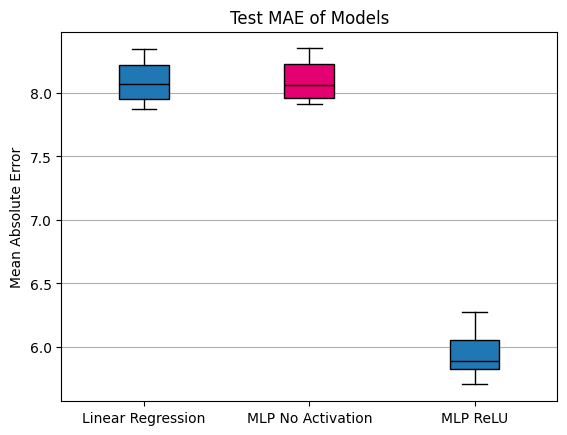
\includegraphics[width=12cm]{./Part II/5.png}
    \caption{Boxplot of the test MAE for each model}
\end{figure}

\item \textbf{Compare a Linear Regression with a MLP with no activations, and explain the impact
and the importance of using activation functions in a MLP. Support your reasoning with the
results from the boxplots.}

\vspace{10pt}
As we can see in the previous plot, the MLP without activation functions behaves similarly to Linear Regression, while the MLP with ReLU activation function performs better than the other two models.
Linear Regression and MLP without activation functions have a high MAE, centered around 8.0. On the other hand, the MLP with ReLU activation function has a lower MAE, centered around 6.0 and this shows the power of activation functions.
Activation functions enable the MLP to learn from non-linear relationships in the data. Without them, each layer is just performing a linear operation, which severely limits the network's ability to generalize and fit real-world data, especially when the underlying relationships are complex or non-linear.

\newpage
\item \textbf{Using a $\mathbf{80-20}$ train-test split with \texttt{random\_state=0}, use a Grid Search to tune the
hyperparameters of an MLP regressor with two hidden layers (size 10 each). The
parameters to search over are: (i) L2 penalty, with the values $\mathbf{\{0.0001, 0.001, 0.01\}}$; (ii)
learning rate, with the values $\mathbf{\{0.001, 0.01, 0.1\}}$; and (iii) batch size, with the values
$\mathbf{\{32, 64, 128\}}$. Plot the test MAE for each combination of hyperparameters, report the
best combination, and discuss the trade-offs between the combinations.}

\vspace{20pt}
\lstinputlisting[language=Python]{./Part II/7.py}

\begin{figure}[h]
    \centering
    % First row with two images side by side
    \begin{subfigure}{0.45\textwidth}
        \centering
        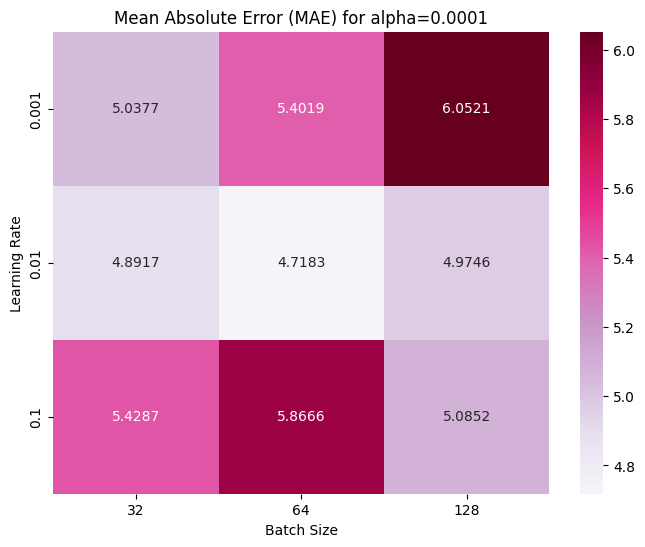
\includegraphics[width=\textwidth]{./Part II/7_1.png}
        \caption{MAE plot for L2 penalty = 0.0001}
    \end{subfigure}
    \hfill
    \begin{subfigure}{0.45\textwidth}
        \centering
        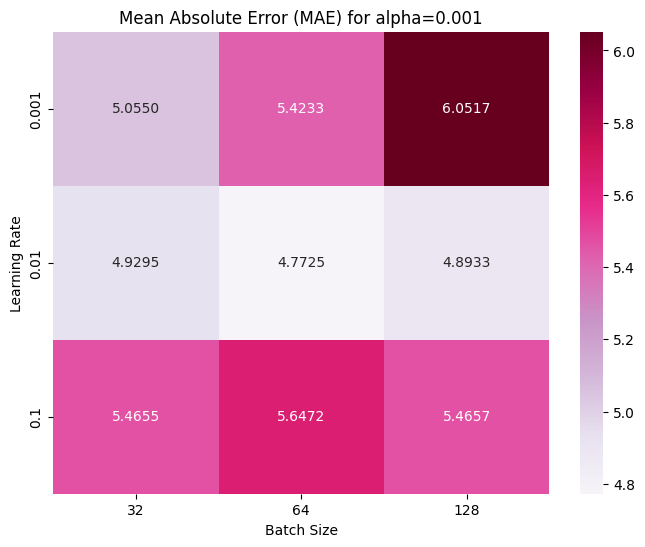
\includegraphics[width=\textwidth]{./Part II/7_2.png}
        \caption{MAE plot for L2 penalty = 0.001}
    \end{subfigure}

    % Space between rows
    \vskip\baselineskip

    % Second row with one image centered
    \begin{subfigure}{0.45\textwidth}
        \centering
        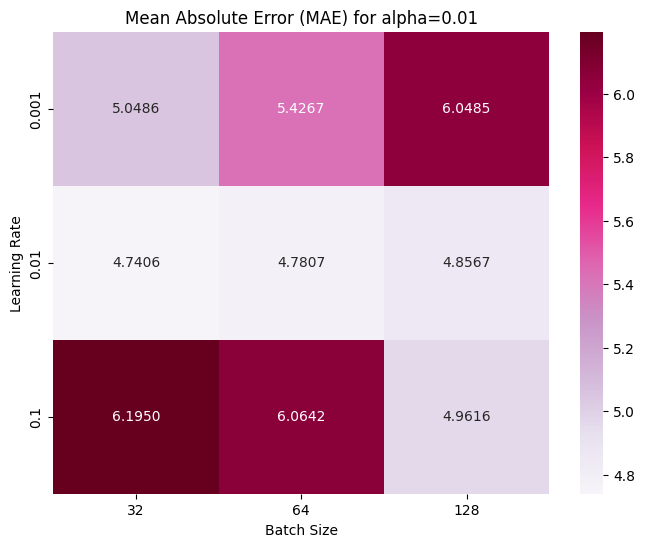
\includegraphics[width=\textwidth]{./Part II/7_3.png}
        \caption{MAE plot for L2 penalty = 0.01}
    \end{subfigure}

    \caption{MAE plot for each combination of hyperparameters}
\end{figure}

\vspace{10pt}
When analizing MAE values (graphics below), the smaller the MAE the better the models performance. With that being said, the best combination for heatmap is:

\begin{itemize}
    \item Learning Rate = 0.01 and Batch Size = 64 for L2 penalty = 0.0001
    \item Learning Rate = 0.01 and Batch Size = 64 for L2 penalty = 0.001
    \item Learning Rate = 0.01 and Batch Size = 32 for L2 penalty = 0.01
\end{itemize}

The best combination of hyperparameters for the MLP regressor, achieving the lowest Mean Absolute Error (MAE) of 4.7183, consists of an L2 penalty (alpha) of 0.0001, a learning rate of 0.01, and a batch size of 64. 
Lower alphas help avoid over-penalizing the model, while the 0.01 learning rate offers a good balance between convergence speed and avoiding overshooting. Batch size 64 provides the best generalization. Higher alphas and learning rates led to higher errors due to over-regularization and poor convergence.

\end{enumerate}

\end{document}
